Für die bereits Eingangs dieses Kapitels gezeigten Schriftarten und Farben:

\begin{quote}

An dieser Stelle sollen exemplarische einige Beispiele gezeigt werden, wie in \LaTeX\ Texte \textbf{Fett}, \textcolor{red}{farbig}, \textit{Kursiv}, \underline{unterstrichen}, \uuline{doppelt unterstrichen}, \uwave{unter\-schlängelt}, \sout{horizontal durchgestrichen}, \xout{schräg durchgestrichen} gesetzt werden und wie Texte formatiert / struk\-tu\-riert werden können.

\end{quote}

ist folgender \LaTeX-Code notwendig: 

\begin{figure}[h!]
    \centering
      \fbox{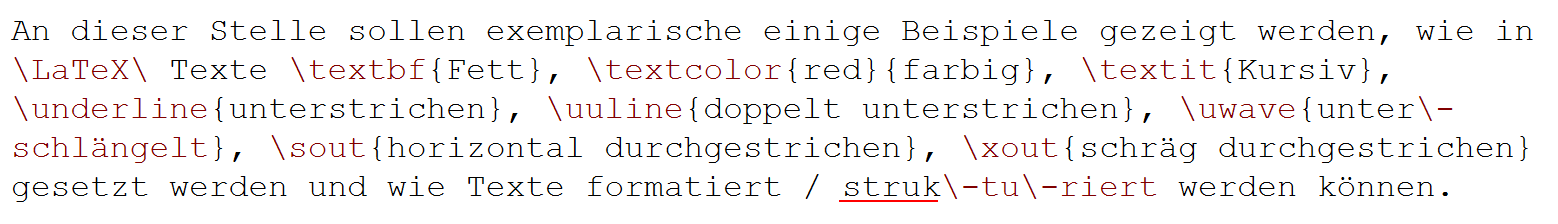
\includegraphics[width=0.75\textwidth]{./Bilder/TextArtenFarben.png}}  
      \caption{Schriftarten und Farben}
\end{figure} 

In diesem Beispiel sieht man auch, wie \LaTeX\ die korrekte Trennung von Wörtern mitgeben kann (siehe die Worte unterschlängelt und strukturiert).
